

\section{Continuation}
\label{sec:continuation}

When the periodic solution is found, finding the successively periodic solutions
for slightly changed parameter values is done by continuation.

A general continuation is formulated as $F(x)=0, \quad
F:\mathbb{R}^{m+1} \to \mathbb{R}^{m} $ where is $F$ the algebraic problem for
which a solution is sought.
For HB, $F$ correspond to $\bm h \in \mathbb{R}^{(2N_H+1)n}$ which depends on
$\bm z \in \mathbb{R}^{(2N_H+1)n}$ and $\omega \in \mathbb{R}^1$; following the
continuation structure. However, as already mentioned, for the shooting method:
$\bm h_{NMM} \in \mathbb{R}^{2n+1}$ which depends on $\bm z \in \mathbb{R}^{2n}$
and $T \in \mathbb{R}^1$; thus not following the structure.
The difference is that with HB, continuation can be done by solving a linear
system using a direct solver, whereas the system is over determined for the
shooting method and a least square solver is needed. It is possible to recast
$\bm h_{NNM}$ into a square problem by adding a artificial parameter
into the Hamiltonian, which during the continuation anyways turns out to be
zero\autocite{detroux2016_phd}. The reason for doing this is that direct
solution is computional faster than iterative solvers.
Note that $\omega$ and $T$ are used interchangeable in this section, ie. by $\bm
h_\omega$ is understood $\bm h_T$ for the shooting method etc..


The most simple continuation method, where $\omega$ is used as independent
parameter and uniformly increased at each step, fails at turning points. Instead
most continuation methods uses a length-wise curve parameter and a
predictor-corrector model. Starting from a known solution $\bm y_j = [\bm
z_{p,(j)},\omega_{(j)}]^T$ the next periodic solution $\bm y_{j+1}$ is found by
the three steps

\begin{itemize}
\item Tangent prediction, $\bm y_{(j+1)}^{(1)} = \bm y_{(j)}+s\bm t_{(i)}$, where
  $s$ is the step size and $\bm t$ the tangent of $\bm y$, ie. the tangent of
  $\bm z_p$ and $\omega$.
\item Newton-like corrections - The type determines the continuation method.
\item Adaptive step control. Here a simple model using the convergence of the
  Newton iterations is used: $s = \frac{it_{opt}}{it_{NR}} s$, ie. the step is
  updated based on a defined optimal number of iterations versus the actual
  used number of iteration
\end{itemize}

The two methods used in this project are the pseudo-archlength- and
the Moore-Penrose continuation. The main difference is computional complexity.
With pseudo-archlength, each time a new point is found on the curve, the tangent
vector have to be computed anew. With the Moore-penrose corrector, the tangent
vector is also corrected and the explicit calculation of the tangent at each new
point is saved.

The aim is to show that is no harder to use the Moore-penrose corrector. Formal
descriptions are found in~\autocite{dhooge2003a}

\subsection{Procedure}
\label{sec:cont_procedure}

The tangent at a solution point $\bm y_{i}$ is
\begin{equation}
  \label{eq:cont_tangent}
  \begin{bmatrix}
    \bm J(\bm y_{(i)}) \\ \bm t^T_{(i-1)}
  \end{bmatrix}
  \bm t_{i}
  =
  \begin{bmatrix}
    \bm 0 \\ 1
  \end{bmatrix}
\end{equation}
where
\begin{equation}
  \label{eq:cont_J}
  \bm J(\bm y_{(i)}) =
  \begin{bmatrix}
    \bm h_{\bm z}(\bm y_{(i)}) & \bm h_{\omega}(\bm y_{(i)})
  \end{bmatrix}
\end{equation}

The last row in eq. \eqref{eq:cont_tangent} prevents the continuation from
turning back, ie. $\bm t^T_{(i-1)} \bm t_{(i)}=1$ and the ``angle of the dot
product'' cannot change sign. For the first tangent calculation the condition is
replaced by a row of ones, which impose the length of the tangent to 1; in later
predictions $\bm t_{(i+1)}$ must be normalized. The prediction is then

\begin{equation}
  \label{eq:cont_pred}
  \bm y^{(1)}_{(i+1)} = \bm y_{(i+1)} + s \bm t_i
\end{equation}

The correction types Pseudo-archlength and Moore-penrose are used with the
shooting method and harmonic balance, respectively. Convergence is achieved when
\begin{equation}
  \label{eq:cont_convergence}
  \frac{\norm{\bm h}}{\norm{\bm z}} < tol
\end{equation}

\subsubsection{Shooting methods}
\label{sec:shooting_cont}

For the pseudo-archlength corrections, a solution is sought in the perpendicular
direction of the prediction. The corrections are given by

\begin{equation}
  \label{eq:nnm_cont_corr}
  \begin{aligned}
    &\bm y^{(j+1)} = \bm y^{(j)} + \Delta \bm y =
    \bm y^{(j)} -\bm G^{-1}_{\bm y} \bm G
  \end{aligned}
\end{equation}
where the prediction subscripts have been omitted. We have
\begin{equation}
  \label{eq:nnm_cont_mat}
    \bm G(\bm y) =
      \begin{bmatrix}
      \bm h_{NNM}(\bm y) \\ \bm 0
    \end{bmatrix}, \quad
    \bm G_{\bm y}(\bm y) =
    \begin{bmatrix}
      \bm J(\bm y) \\ \bm t^T
    \end{bmatrix}
  \end{equation}
where correction superscripts have been omitted. After convergence to a
solution, the tangent is calculated and the algorithm continues.

The phase condition $g(\bm z)$, as seen in eq. \eqref{eq:sm_nr_sol}, should
formally be included in eqs. \eqref{eq:cont_tangent}-\eqref{eq:nnm_cont_mat},
ie. in the predictions one adds the equation $ \begin{bmatrix}g_{\bm z} &
  0 \end{bmatrix} \bm t_i = 0 $ and in the corrections $ \begin{bmatrix}g_{\bm
    z} & 0 \end{bmatrix} \bm t_i = - g(\bm z) $. But instead of adding
conditions, it is used that NNMs for all practical circumstances are symmetric,
the loss of symmetry requires a symmetry breaking bifurcation
\autocite{kerschen2009b}, ie. the initial velocity is zero for all dofs. Thus
the velocities can be removed from the unknowns and the system to solve then
have $2n+1$ equations with $n+1$ unknowns.


\subsubsection{Harmonic balance}
\label{sec:hb_cont}

For the Moore-penrose corrections, the nearest solution to the prediction is
sought. This is done by updating the tangent direction at each corrector
iteration.

Using a optimisation variable $\bm v$, initialised as the prediction tangent
$\bm v^{(1)} = \bm t_{(i)}$, the Moore-penrose corrections are given by

\begin{equation}
  \label{eq:hb_cont_corr}
  \begin{aligned}
    &\bm y^{(j+1)} = \bm y^{(j)} + \Delta \bm y =
    \bm y^{(j)} -\bm G^{-1}_{\bm y} \bm G \\
    &\bm v^{(j+1)} = \bm v^{(j)} + \Delta \bm y =
    \bm v^{(j)} -\bm G^{-1}_{\bm y} \bm R
  \end{aligned}
\end{equation}
where the prediction subscripts have been omitted. We have
\begin{equation}
  \label{eq:hb_cont_mat}
  \begin{gathered}
    \bm G(\bm y, \bm v) =
    \begin{bmatrix}
      \bm h(\bm y) \\ \bm 0
    \end{bmatrix}, \quad
    \bm G_{\bm y}(\bm y, \bm v) =
    \begin{bmatrix}
      \bm J(\bm y) \\ \bm v^T
    \end{bmatrix} \\
      \bm R(\bm y, \bm v) =
  \begin{bmatrix}
    \bm J(\bm y) \bm v \\ \bm 0
  \end{bmatrix}
  \end{gathered}
\end{equation}
where correction superscripts have been omitted.

When convergence is reached the tangent is calculated as the normalized
correction of $\bm v$, $\bm t_{(j+1)} = \frac{\bm v}{\norm{\bm v}}$.

During the corrections eq. (\ref{eq:hb_cont_corr}-\ref{eq:hb_cont_mat}) $\bm h_{\bm
  z}$ is calculated, making stability analysis with Hills method cheap after
each solution is obtained.

As a final note, $\bm h_\omega$ in the jacobian eq. \eqref{eq:cont_J} is given by
\begin{equation}
  \label{eq:hb_cont_Hw}
  \bm h_\omega = \frac{\p \bm A}{\p \omega} \bm z
\end{equation}

\subsection{Example}
\label{sec:cont_example}

\subsubsection{NNM}

Figure \ref{fig:nnm_2dof} shows the two NNMs, the in-phase and out-of-phase, for
the coupled duffing system \eqref{eq:2dof} in a frequency-energy plot(FEP).
The evolution of natural frequencies are seen wrt. to the total energy of the
system. At low energy the NNM frequencies are close to the linear frequencies,
but as energy increases, the natural frequency increases due to the cubic
nonlinear hardening. As the energy increases, the two NNMs coincide and it is
not possible to obtain commensurate ratio between the two natural frequencies.
Thus there is no internal resonance.

The insert shows the configuration space, and it seen that both branches of NNMs
have straight modal lines, which is due to the symmetry of the system: due to
the symmetry there are only similar NNMs.


\begin{figure}[!ht]
  \centering
  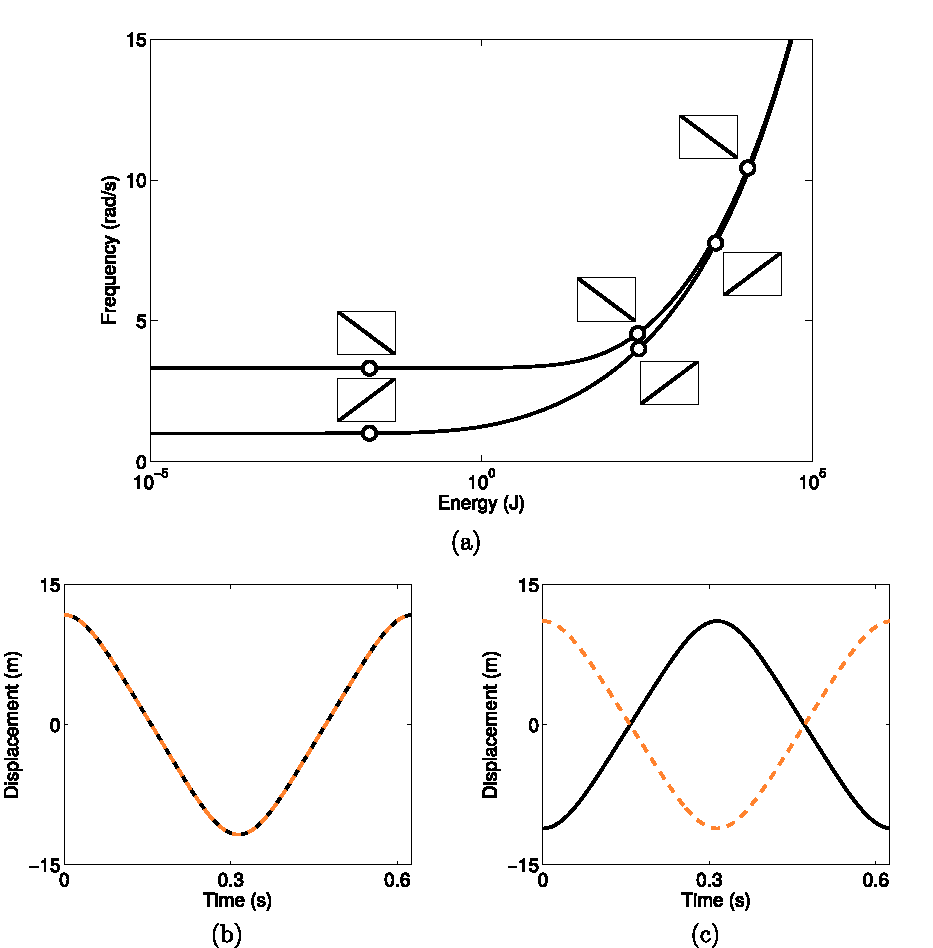
\includegraphics[width=0.7\linewidth]{continuation/nnm_2dof.pdf}
  \caption{NNMs for the coupled duffing system \eqref{eq:2dof}.
    \textbf{(a)}: Frequency-energy plot(FEP). NNM motion(configuration space,
    ie. $x_1$ vs. $x_1$) at given frequencies are shown in inserts;
    \textbf{(b)}: in-phase NNM at $\omega=10$rad/s;
    \textbf{(c)}: out-of-phase NNM at $\omega=10$rad/s;
    \sampleline{}: $x_1$;
    \textcolor{orange}{\sampleline{dashed}}: $x_2$.
  }
  \label{fig:nnm_2dof}
 \end{figure}


\subsubsection{HB}

Figure \ref{fig:hb_frf_2dof} shows the NRFC for the coupled duffing using five
harmonic terms, which is enough to capture the harmonic components as seen in
figure \ref{fig:hb_duffing_periodic}.
If a lower number of harmonic were
included - only one and three terms would be relevant since even harmonics are
zero; it would required an even nonlinearity to generate even harmonics - the
superharmonic resonances at lower frequencies will not be captured. See appendix
\ref{sec:hb_appendix} where NRFCs are shown for different HB and continuation
parameters.

\begin{figure}[!ht]
  \centering
  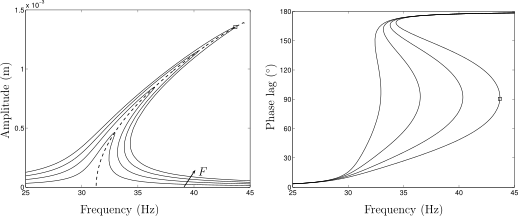
\includegraphics[width=0.7\linewidth, height=8cm]{2dof_duffing/nfrc}
  \caption{NRFC of the coupled duffing system \eqref{eq:2dof} for $x_1$ with
    $f=2$N. Unstable motion are indicated by $- - -$. $N_H = 5, N = 512$.
    Markers indicate amplitudes for a stepped sine.
    $\times$: increasing;
    \textcolor{red}{$\circ$}: decreasing.}
  \label{fig:hb_frf_2dof}
 \end{figure}

\subsection{Summary}
\label{sec:cont_summary}

Figure \ref{fig:cont_algo} show an algorithm for the continuation procedure,
regardless of the the correction method. There is not much difference if
implementation complexity of the two corrections, but the Moore-penrose
corrections saves on computional complexity. The Pseudo-arclength method can be
seen as a Moore-Penrose method for which the correction direction is not
updated.

\begin{figure}[!ht]
  \centering
  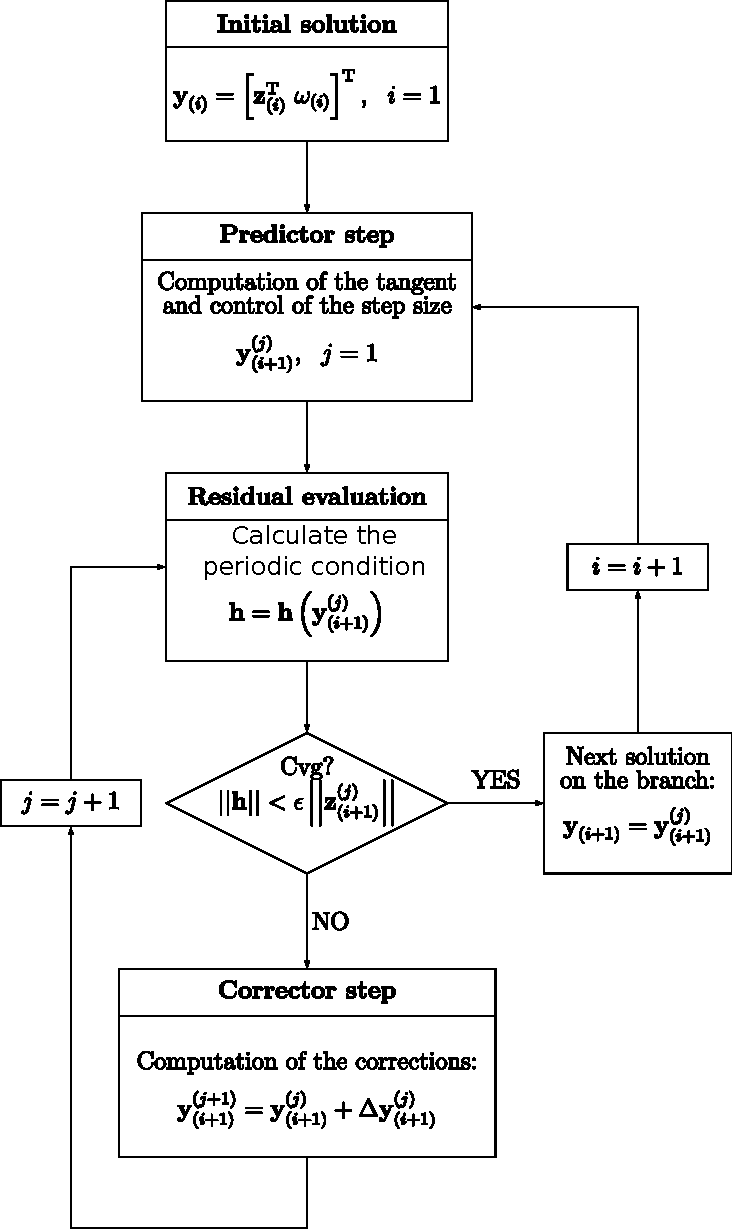
\includegraphics[width=0.7\textwidth]{continuation/continuation_diagram}
  \caption{Algorithm for Predictor-Corrector continuation of a periodic
    solution. For Moore-penrose the successive tangents are simply calculated as
  a normalization.}
  \label{fig:cont_algo}
\end{figure}



%%% Local Variables:
%%% mode: latex
%%% TeX-master: "../../report"
%%% End:
